\documentclass[11pt,a4paper]{article}
\usepackage[margin=25mm,headheight=14pt]{geometry}
\usepackage[T1]{fontenc}
\usepackage{lmodern}
\usepackage{microtype}
\usepackage{amsmath,amssymb,booktabs,graphicx,float}
\usepackage[font=small,labelfont=bf]{caption}
\usepackage{fancyhdr,lastpage}
\usepackage{hyperref}
\usepackage{xurl}
\hypersetup{colorlinks=true,linkcolor=black,urlcolor=blue,citecolor=black}
\setlength{\parindent}{1.5em}
\setlength{\parskip}{0.25em}
\pagestyle{fancy}
\fancyhf{}
\fancyhead[L]{Team \underline{\hspace{12mm}} \quad Problem A}
\fancyhead[R]{Page \thepage\ of \pageref{LastPage}}
\fancyfoot[C]{\thepage}
\renewcommand{\headrulewidth}{0.4pt}

\begin{document}
\thispagestyle{empty}
\begin{center}
{\Large\bfseries How High Can a Space Diver Safely Descend?}\\[8pt]
{\normalsize Team number: \underline{\hspace{30mm}}\qquad Problem A}\\[15pt]
{\large\bfseries Summary}
\end{center}

For a 190\,kg suited diver and parachute system, mass alone does not determine a survivable exit altitude. Drag area, stability control, suit heat tolerance, parachute deployment, and human loads must also be specified. We construct a reproducible vertical model using the 1976 U.S. Standard Atmosphere, variable gravity, and a staged canopy. Its freefall drag area is fitted to the March and July 2012 Stratos peak speeds; the October speed is withheld from fitting. The October prediction is 354.3\,m\,s$^{-1}$ against 377.1\,m\,s$^{-1}$ observed (6.1\% low), while peak time is 49.0\,s against approximately 50\,s. A separate fit to Alan Eustace's drogue-assisted jump predicts peak time 50.2\,s against 51\,s reported. These sparse flight checks constrain vertical dynamics but do not validate a high-altitude survival limit.

With the fitted drag area transferred to 190\,kg, a 60\,km exit yields 639\,m\,s$^{-1}$ peak speed, 6.13\,kPa peak dynamic pressure, and 416\,K recovery-temperature proxy; a stagnation-temperature proxy reaches 438\,K. An illustrative 100\,m$^2$ canopy drag area inflated over 8\,s gives 4.41\,$g$ modeled aerodynamic proper acceleration and 5.52\,m\,s$^{-1}$ sea-level landing speed. Neither is a certified opening or landing performance. If assumed equipment screens of 6\,kPa and 400\,K are imposed, the fitted case crosses at 57.7\,km. Effective drag areas inferred separately from the three Stratos flights move this conditional screen to 42.7--57.8\,km. Thermal-proxy choice shifts it again. As these thresholds and spin control lack applicable qualification data, no universal maximum can be inferred from 190\,kg.

\newpage
\tableofcontents
\newpage

\section{Problem and scope}
The 2023 University Physics Competition Problem A asks for challenges, dangers, and the maximum altitude for a vertical rocket-exit descent with total mass 190\,kg \cite{problem}. This manuscript follows the supplied Tongji Team 355 paper's A4, single-column structure: centered first-page title and summary, contents, assumptions, symbols, model, calculations, discussion, and references \cite{tongji}. Its text, calculations, and plots are newly prepared. The competition's current rules require a first page containing only the team number, problem, title, and summary; the submission team number is intentionally blank here \cite{rules}.

The word \emph{successfully} includes more than reaching the ground. A viable sequence needs controlled orientation, an intact suit and life-support system, acceptable heat and pressure exposure, a canopy that can open at a suitable altitude and airspeed, tolerable opening acceleration, and a survivable landing. We therefore distinguish a dynamical feasibility screen from a verified human and hardware safety bound.

\section{Prior approaches and the missing constraints}
Table~\ref{tab:prior} compares published 2023 Problem A solutions. Their answers differ largely because each assigns different limiting mechanisms or hardware thresholds. The Team 355 spin-endurance criterion integrates drag acceleration over time and compares it with a scaled historical value; the integral has units of velocity, so it cannot alone represent angular spin without a torque, moment arm, inertia, and control model. We retain its attention to spin as a hazard but do not use that criterion as an empirical safety threshold.

\begin{table}[H]\centering\small
\caption{Selected published Problem A results and their dominant assumed limitation. They are modeling precedents, not independent validation data.}
\label{tab:prior}
\begin{tabular}{p{18mm}p{25mm}p{91mm}}\toprule
Team & Reported scale & Principal modeling choice \\\midrule
355 & 57\,km & Drag-based spin endurance proxy \cite{tongji}\\
244 & 61.27\,km & Suit heating threshold \cite{team244}\\
447 & 63.78\,km & Thermal limit; much higher opening-only bound \cite{team447}\\
464 & 60.675\,km & Thermal limit under its suit assumptions \cite{team464}\\
131 & about 80--94\,km & Spin and other constraints change the answer \cite{team131}\\
227 & 153\,km & Assumed parachute heat resistance \cite{team227}\\\bottomrule
\end{tabular}
\end{table}

The numerical span is evidence of an underdetermined design problem. The combined 190\,kg mass fixes inertia only after the body's geometry is supplied, and drag only after area and coefficient are supplied. Suit and parachute ratings are design inputs, not consequences of mass.

\section{Assumptions and notation}
\begin{enumerate}
\item The rocket is at apogee when the diver exits, with approximately zero velocity relative to a windless local atmosphere. The diver follows a one-dimensional vertical path. This excludes winds, tumbling, lift, and line twist.
\item The 1976 U.S. Standard Atmosphere specifies temperature and density to 86\,km \cite{ussa}. It is a reference profile, not weather from a particular jump day. All altitude sweeps stop at 80\,km.
\item Freefall uses an effective constant drag area $C_DA$, represented by ballistic coefficient $\beta=m/(C_DA)$. This averages changing posture and Mach-dependent drag; its extrapolation is a major uncertainty.
\item The illustrative main canopy starts deployment at the Stratos final-jump main-parachute pull altitude, 2566.8\,m above mean sea level. The modeled landing surface is sea level, so this is not a reconstruction of the Stratos landing terrain. Canopy drag area rises smoothly to 100\,m$^2$ over either 4 or 8\,s. A real deployment would need a staged reefing and inflation design.
\item The entire person--suit--oxygen--parachute assembly has mass 190\,kg. A 100\,m$^2$ canopy effective drag area is only a mathematical scenario; its fabric, lines, reserve system, and life support have not been shown to fit that mass budget.
\item Thermal exposure is summarized only by a perfect-gas adiabatic wall-temperature proxy. It is not a suit-skin, parachute-fabric, or body temperature prediction.
\end{enumerate}

\begin{table}[H]\centering\small
\caption{Symbols used in the reduced-order model.}
\begin{tabular}{lll}\toprule
Symbol & Meaning & Unit\\\midrule
$h,v$ & Geometric altitude; downward speed & m; m\,s$^{-1}$\\
$m,\beta$ & Total mass; ballistic coefficient & kg; kg\,m$^{-2}$\\
$\rho,T,a$ & Air density, temperature, sound speed & kg\,m$^{-3}$; K; m\,s$^{-1}$\\
$q$ & Dynamic pressure, $\rho v^2/2$ & Pa\\
$a_{\rm p}$ & Proper acceleration from aerodynamic force & m\,s$^{-2}$\\
$T_{\rm aw}$ & Adiabatic wall-temperature proxy & K\\
$\tau,C_DA_c$ & Canopy inflation time, full drag area & s; m$^2$\\\bottomrule
\end{tabular}
\end{table}

\section{Model}
\subsection{Atmosphere and freefall}
The program evaluates the 1976 standard-atmosphere geopotential layers, converting geometric altitude $h$ to geopotential height $z=R_Eh/(R_E+h)$ and obtaining $\rho=p/(R_{\rm air}T)$. Sound speed is $a=\sqrt{\gamma R_{\rm air}T}$. With downward speed positive,
\begin{align}
\dot h&=-v,\\
\dot v&=g_0\left(\frac{R_E}{R_E+h}\right)^2-\frac{\rho(h)v|v|}{2\beta},
\qquad
\beta=\frac{m}{C_DA}.
\label{eq:motion}
\end{align}
The model computes $M=v/a$ and $q=\rho v^2/2$. Freefall proper acceleration is $a_{\rm p}=qC_DA/m=q/\beta$. A small proper acceleration immediately after exit is expected even though gravitational acceleration remains near $g$.

For a heating \emph{screen}, we calculate both turbulent-flow recovery temperature and the ideal stagnation temperature:
\begin{equation}
T_{\rm aw}=T\left(1+r\frac{\gamma-1}{2}M^2\right),\qquad
r=\mathrm{Pr}^{1/3}\simeq 0.89,\quad \mathrm{Pr}=0.71,
\qquad T_0=T+\frac{v^2}{2c_p}.
\label{eq:heat}
\end{equation}
The two proxies differ at exposed locations: a nominal stagnation point can approach $T_0$, while recovery along a turbulent surface uses $T_{\rm aw}$. Neither determines heat flux, exposure duration, conduction through layers, or actual suit temperature. Both become especially questionable at low density and supersonic speed. A thermal crossing derived from either is explicitly conditional.

\subsection{Parachute phase}
At the selected opening altitude the model continues Eq.~\eqref{eq:motion}, replacing $C_DA$ by
\begin{equation}
\begin{aligned}
C_DA(t)&=C_DA_{\rm free}
 +\bigl(C_DA_c-C_DA_{\rm free}\bigr)S(x),\\
S(x)&=3x^2-2x^3,\qquad
x=\max\left(0,\min\left[1,\frac{t-t_{\rm open}}{\tau}\right]\right).
\end{aligned}
\label{eq:canopy}
\end{equation}
For a nominal sea-level terminal-speed target of 5.5\,m\,s$^{-1}$, the steady-force balance gives
\begin{equation}
(C_DA)_c \simeq \frac{2mg_0}{\rho_0v_{\rm target}^2}
=\frac{2(190)(9.80665)}{(1.225)(5.5)^2}
\simeq 100\ {\rm m^2}.
\label{eq:canopysize}
\end{equation}
The target is an illustrative design input, not a certified injury threshold. Effective drag area is not fabric area, and no canopy or line mass is inferred from this calculation.
The resulting $a_{\rm p}=q C_DA(t)/m$ is the modeled \emph{total aerodynamic proper acceleration}; net downward acceleration is $g-a_{\rm p}$. It is not the harness line load, which depends on canopy forces and inflation transients. Snatch force, added air mass, and inflation overshoot are absent. The airspeed and local pressure at opening must also be checked against the actual parachute's certified deployment envelope. NASA parachute engineering treats peak opening load as a separate design quantity, although the cited study concerns Mars parachutes rather than personnel equipment \cite{nasaopen}. The smooth inflation law is a transparent scenario, not a parachute qualification model.

\section{Calibration and validation against existing flights}
\subsection{Data provenance and split}
The Stratos scientific summit report gives summarized measured values for three 2012 jumps \cite{stratos}. These are not raw GPS or accelerometer samples. The peer-reviewed Stratos analysis reports a suited mass of 121.2\,kg and changing projected area and drag with posture and Mach number \cite{guerster}. Its data originate from the same mission, so it is supporting interpretation rather than an independent flight. We fit one freefall $\beta$ to March and July peak speeds; the October \emph{speed record} is not used in that fit and is reserved for a check. The 121.2\,kg mass, however, comes from the October analysis and is a physical-input estimate rather than a blinded parameter. We then transfer the fitted \emph{drag area}, not the fitted $\beta$, to 190\,kg:
\begin{equation}
(C_DA)_{\rm fit}=\frac{121.2}{148.87}=0.8142~{\rm m^2},
\qquad
\beta_{190}=\frac{190}{0.8142}=233.37~{\rm kg\,m^{-2}}.
\label{eq:transfer}
\end{equation}
This transfer is a declared shape assumption. A heavier suit, changed posture, or stabilizing device could alter the drag area.

\begin{table}[H]\centering\small
\caption{Measured mission summaries and freefall-model predictions. March and July peak speeds are calibration inputs; October is held out. Low-$g$ means published duration below 0.1\,$g$ proper acceleration.}
\label{tab:validation}
\begin{tabular}{lrrrrr}\toprule
2012 flight & Exit (km) & Peak observed & Peak modeled & Low-$g$ observed & Low-$g$ modeled\\
 & & \multicolumn{2}{c}{(m\,s$^{-1}$)} & \multicolumn{2}{c}{(s)}\\\midrule
March 15 & 21.828 & 163.0 & 162.1 & 6.1 & 7.0\\
July 25 & 29.610 & 241.5 & 243.2 & 9.3 & 12.3\\
October 14 & 38.969 & 377.1 & 354.3 & 25.2 & 22.3\\\bottomrule
\end{tabular}
\end{table}

The October peak-speed relative error is $-6.1\%$; its modeled peak occurs at 49.0\,s versus about 50\,s reported. The predicted first sound-speed crossing is 34.8\,s versus 34\,s reported, and its return below sound speed is 64.9\,s versus 64\,s \cite{stratos}. Agreement in timing does not erase the peak-speed error: a fixed effective drag area misses altitude, Mach, and body-position effects. The larger July low-$g$ discrepancy is a visible model limitation. We do not fit any safety threshold to these data.

\begin{figure}[H]\centering
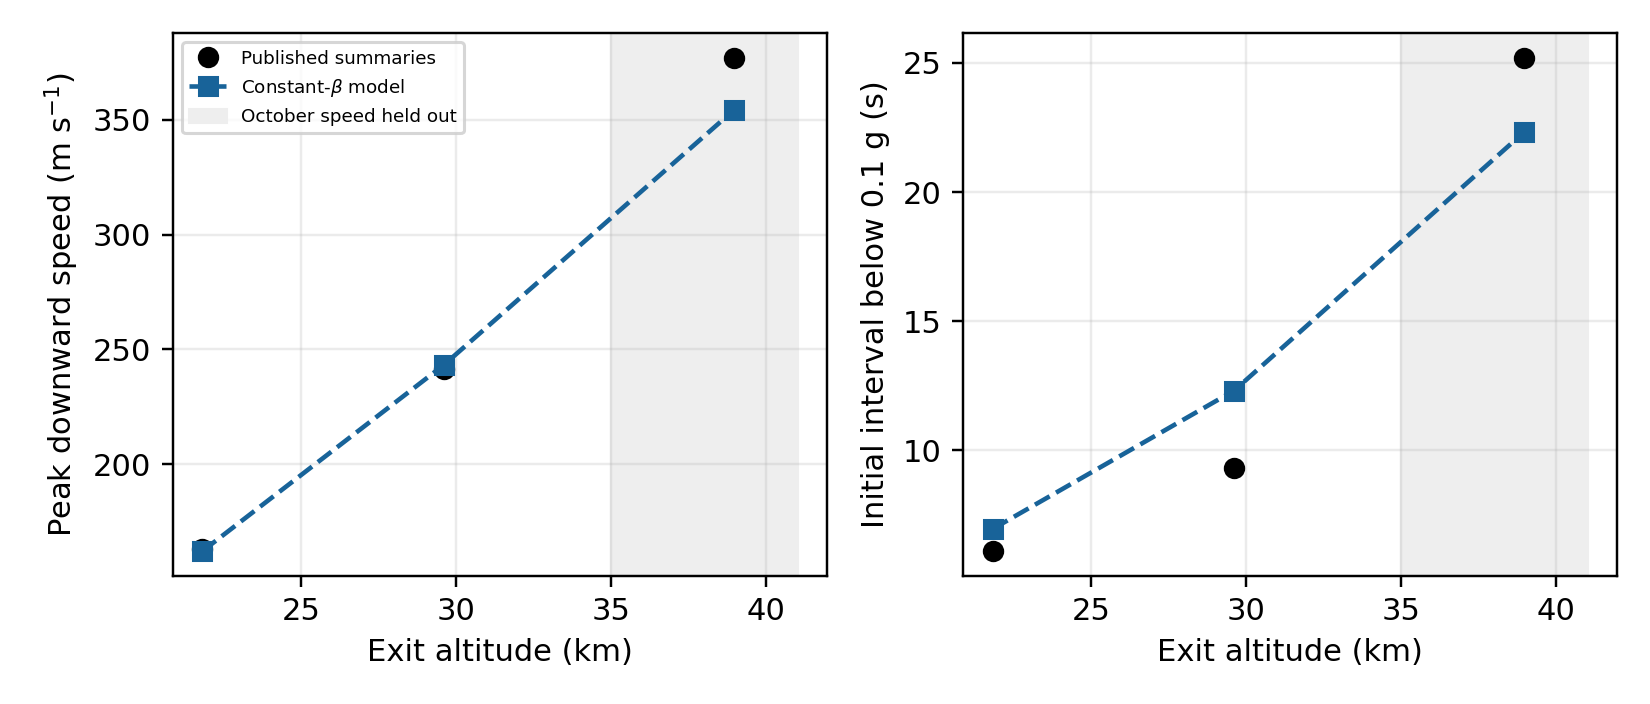
\includegraphics[width=.84\linewidth]{figures/flight_validation.png}
\caption{Model versus published Stratos peak speeds and initial low-acceleration intervals. Only the March and July peak speeds calibrate the central $\beta$; the October speed and all low-$g$ durations are checks. Observations are published summaries, not reconstructed telemetry.}
\end{figure}

Alan Eustace's 2014 flight supplies a second mission with approximately 200\,kg person-plus-equipment mass, 41.422\,km exit altitude, 1320\,km\,h$^{-1}$ peak speed after 51\,s, and Mach 1 after 35\,s \cite{fai}. His drogue-assisted geometry differs from the Stratos freefall configuration. Fitting a separate effective $\beta=119.24$\,kg\,m$^{-2}$ to the published peak speed predicts peak time 50.2\,s and first Mach 1 at 34.8\,s. This checks timing within a different descent regime; because speed was used for fitting and the effective drag was changed, it is not an independent 190\,kg high-altitude validation.

After the held-out check, we solve for a separate effective drag area from \emph{each} Stratos peak speed to diagnose flight-to-flight variation (Table~\ref{tab:cda}). The October value is much smaller; posture and transonic drag changes are plausible causes, but a single peak speed cannot isolate them. These individual values are \emph{not} put back into the original March--July calibration. We use their spread below only as empirical sensitivity scenarios, not as a confidence interval.

\begin{table}[H]\centering\small
\caption{One-event effective drag-area estimates using the published peak speeds and 121.2\,kg mass. Each is the $C_DA$ that reproduces that event's peak speed in the one-dimensional model.}
\label{tab:cda}
\begin{tabular}{lrrr}\toprule
Stratos flight & March 15 & July 25 & October 14\\\midrule
Inferred $C_DA$ (m$^2$) & 0.801 & 0.834 & 0.612\\\bottomrule
\end{tabular}
\end{table}

\subsection{Independent measured-atmosphere check}
The standard atmosphere is a climatological reference, not the atmosphere on any jump day. To test its local applicability where observations exist, we obtained eight dated radiosonde profiles from the University of Wyoming upper-air archive: Santa Teresa station 72364 and Albuquerque station 72365 on the March, July, and October Stratos dates, with an additional 00Z profile following October 14 \cite{wyoming}. The cleaned level data, source URLs, and response hashes accompany the calculation. Profiles measure pressure and temperature versus \emph{geopotential} height; at 10, 20, and 25\,km we interpolate temperature linearly and pressure logarithmically, then compute density from $p/(R_{\rm air}T)$. This is a comparison against a separate observing system, not another fit of $\beta$.

\begin{table}[H]\centering\small
\caption{Nearby October 14, 2012 12Z radiosondes versus the 1976 reference atmosphere. Density deviation is $(\rho_{\rm obs}/\rho_{\rm std}-1)\times100\%$ at fixed geopotential height.}
\label{tab:sounding}
\begin{tabular}{lrrr}\toprule
Station & Height (km) & $T_{\rm obs}-T_{\rm std}$ (K) & Density deviation (\%)\\\midrule
Santa Teresa & 10 & +8.18 & +2.74\\
Santa Teresa & 20 & $-8.94$ & +6.48\\
Santa Teresa & 25 & $-5.01$ & +2.58\\
Albuquerque & 10 & +6.57 & +2.66\\
Albuquerque & 20 & $-7.28$ & +5.76\\
Albuquerque & 25 & $-4.20$ & +2.20\\\bottomrule
\end{tabular}
\end{table}

The stations lie approximately 259 and 273\,km from the Roswell airport reference point. Their October 12Z profiles end at 25.97 and 30.62\,km, respectively; they do not observe the 33\,km speed maximum of the illustrative 60\,km descent, much less the 60--80\,km release region. Figure~\ref{fig:sounding} shows that the reference temperature misses some vertical structure even where density differences at selected levels remain a few percent. The atmospheric comparison therefore checks only the lower observed layers and does not validate high-altitude heating or the entire trajectory.

\begin{figure}[H]\centering
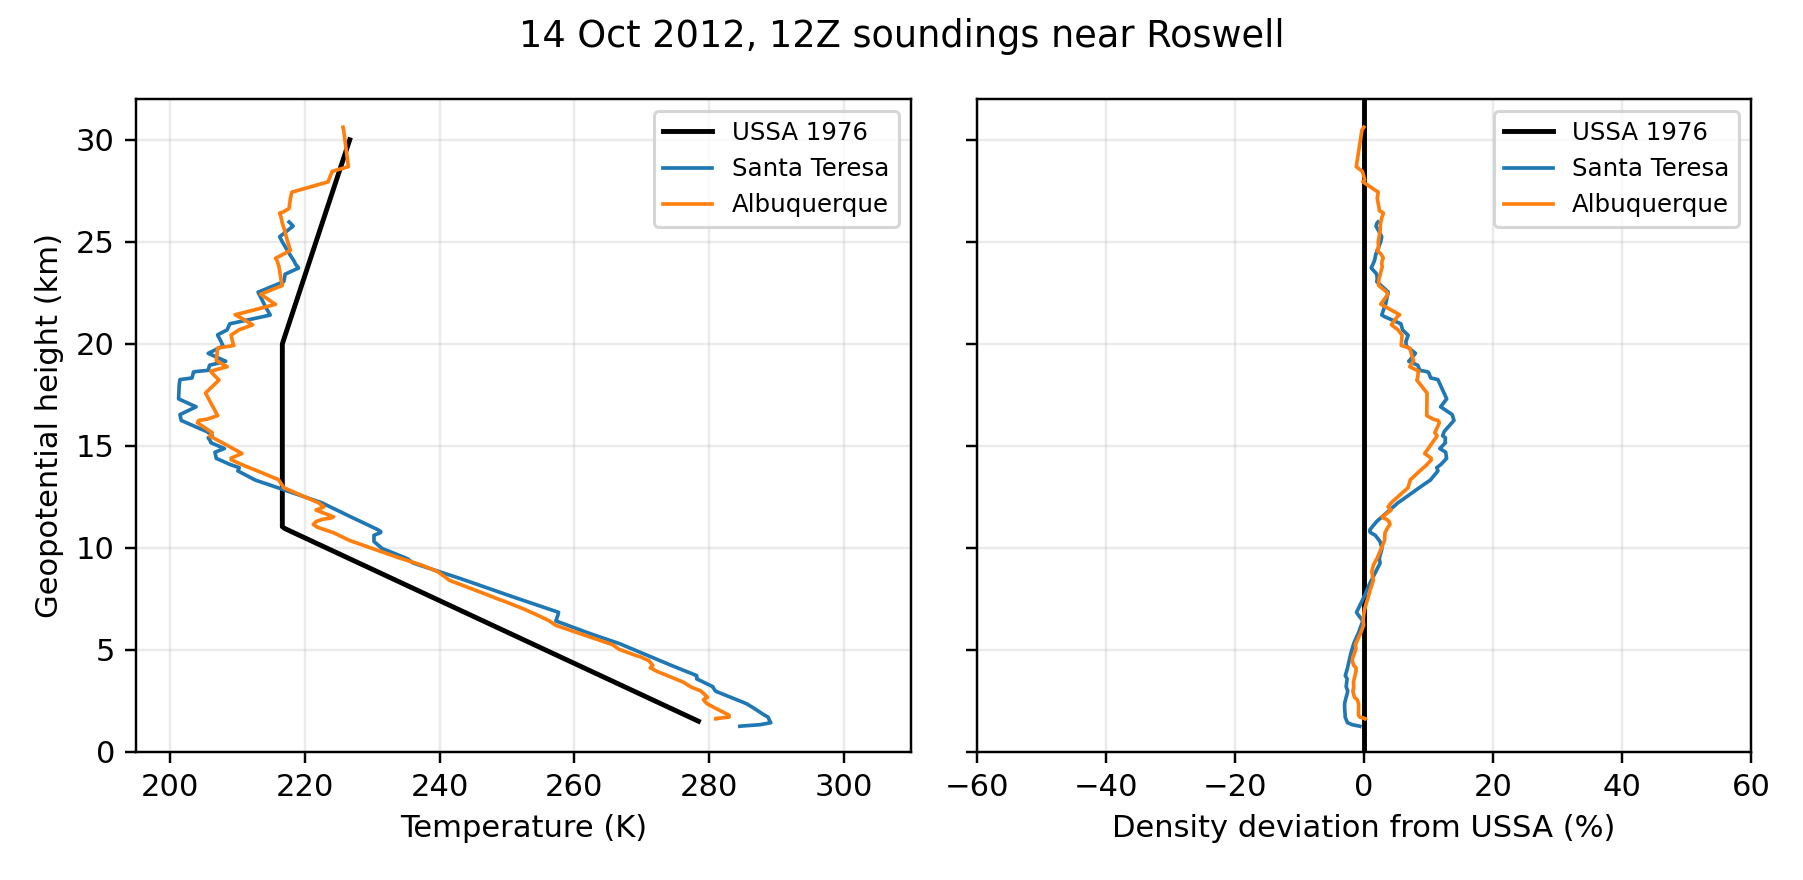
\includegraphics[width=.82\linewidth]{figures/sounding_validation.png}
\caption{Measured October 14, 2012 12Z soundings and the 1976 reference profile. Left: temperature. Right: observed density deviation from the reference. The source stations are nearby, not on the Stratos flight path.}
\label{fig:sounding}
\end{figure}

\section{A 190 kg scenario and conditional altitude screen}
\subsection{Descent and canopy loads}
At 60\,km exit, the transferred freefall drag area gives 638.9\,m\,s$^{-1}$ peak speed at 33.26\,km, 6.13\,kPa peak dynamic pressure, 415.7\,K maximum $T_{\rm aw}$, and 437.6\,K maximum $T_0$. Maximum Mach number is approximately 2.1, well beyond the approximately Mach 1.25 range sampled by the October Stratos jump \cite{guerster}. These maxima occur at different points and must not be combined as if simultaneous. Near 2566.8\,m main-parachute pull altitude, the modeled freefall speed is 70.3\,m\,s$^{-1}$. Table~\ref{tab:canopy} shows how the assumed inflation time changes total aerodynamic proper acceleration; both cases approach 5.52\,m\,s$^{-1}$ sea-level landing speed. Neither the needed canopy system nor this landing speed is shown safe for the 190\,kg assembly.

\begin{table}[H]\centering\small
\caption{Illustrative 60\,km exit and 100\,m$^2$ canopy drag-area scenarios. The peak proper acceleration is the modeled total aerodynamic force divided by $mg_0$, not a measured harness shock.}
\label{tab:canopy}
\begin{tabular}{lrrr}\toprule
Inflation time (s) & Opening speed (m\,s$^{-1}$) & Peak proper load ($g_0$) & Landing speed (m\,s$^{-1}$)\\\midrule
4 & 70.28 & 6.48 & 5.52\\
8 & 70.28 & 4.41 & 5.52\\\bottomrule
\end{tabular}
\end{table}

In the 8\,s case, the computed fall takes approximately 243\,s to reach the main-parachute pull altitude and a further 418\,s to land at the hypothetical sea-level surface: about 11.0\,min in total. Oxygen, pressure regulation, cooling, and backups must operate throughout this interval with reserve. The 190\,kg budget has not been partitioned into person, suit, gas supply, main and reserve canopies, and lines.

\begin{figure}[H]\centering
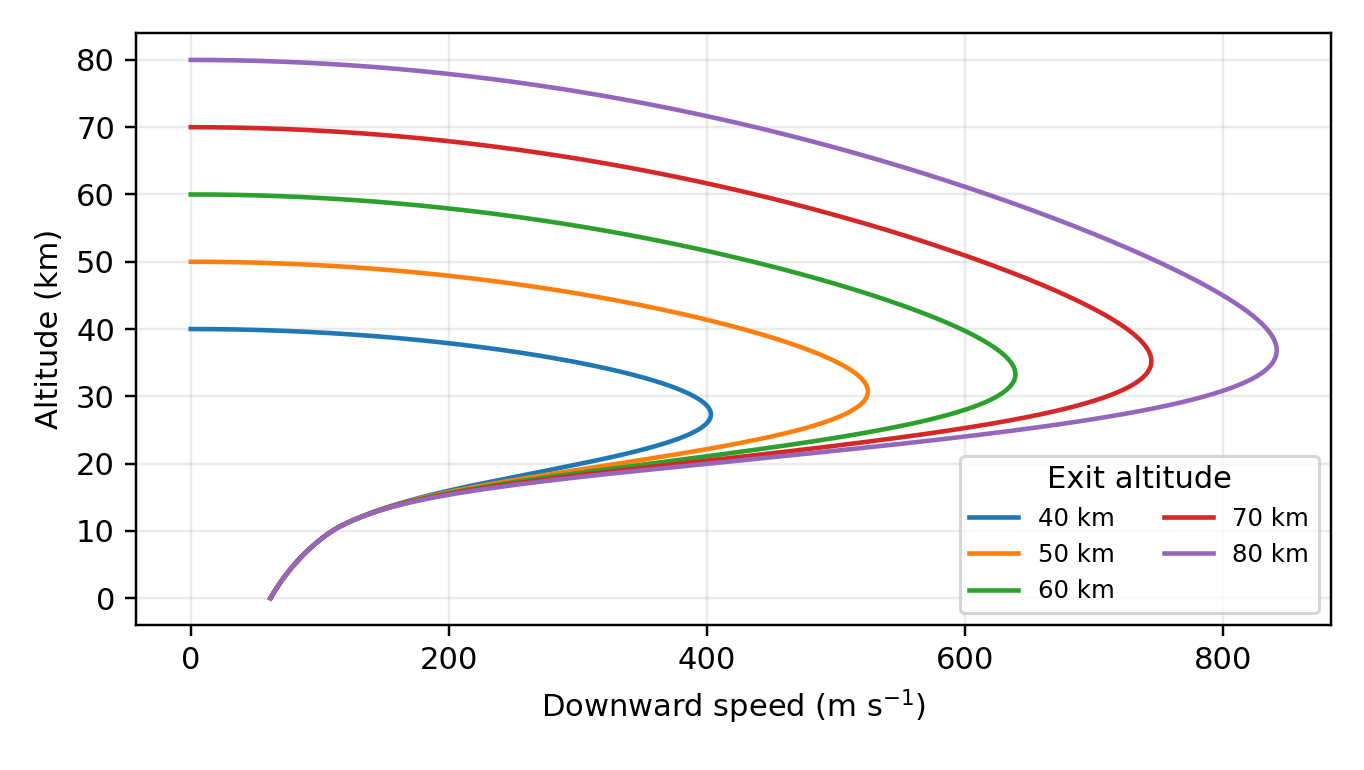
\includegraphics[width=.84\linewidth]{figures/speed_altitude.png}
\caption{Illustrative 190\,kg freefall speed versus altitude for multiple release heights. Curves use the same transferred effective drag area.}
\end{figure}

\subsection{Why a unique maximum is unavailable}
For a specified design, a maximum altitude would be the largest $H$ satisfying \emph{all} constraints, for example
\begin{equation}
\begin{aligned}
H_{\max}(\mathcal D)=\sup\{H:\;&
q_{\max}(H)\le q_{\rm allow},\
T_{\rm suit,max}(H)\le T_{\rm allow},\\
&
a_{\rm open,max}(H)\le a_{\rm allow},\
\text{other safety checks pass}\}.
\end{aligned}
\label{eq:bound}
\end{equation}
Here $\mathcal D$ denotes the equipment and physiological specification. Neither $q_{\rm allow}$ nor a suit temperature limit is given by the problem. More importantly, $T_{\rm suit,max}$ is not computed by Eq.~\eqref{eq:heat}. Stability cannot be inferred from vertical speed alone. Published reports discuss the danger of uncontrolled flat spin and actual spin in a stratospheric jump \cite{spin,stratos}; a real bound requires angular-dynamics and control testing. Suit pressure, oxygen duration, decompression, and visor integrity need separate specifications. NASA's human-system standards make clear that acceleration tolerance depends on axis, duration, and restraint, rather than on a single universal $g$ number \cite{nasahuman}.

To make the sensitivity concrete, we temporarily use $q_{\rm allow}=6$\,kPa and $T_{\rm aw,allow}=400$\,K as \emph{assumed equipment-screen values}. The pressure limit would imply approximately 2.62\,$g$ body aerodynamic proper load at the fitted $C_DA$, but $q$ itself is not a human injury metric. Neither value is a certified suit, helmet, or parachute rating. Linear interpolation of the computed 5\,km grid gives a pressure crossing at 58.8\,km and recovery-temperature crossing at 57.7\,km; their minimum is 57.7\,km for the central drag-area fit. If the same 400\,K marker is applied instead to the stagnation proxy $T_0$, its central crossing becomes 55.0\,km. This does not establish a thermal failure temperature; it measures model-definition sensitivity.

Table~\ref{tab:screen} repeats the \emph{same hypothetical thresholds} after transferring each observed flight's one-event effective drag area to 190\,kg. The joint screen ranges from 42.7 to 57.8\,km. In particular, a smaller area produces higher dynamic pressure and moves the assumed pressure crossing sharply downward. The range is neither a probability interval nor a verified survivable-altitude range: the three fits are sparse, correlated by equipment, and extrapolated far beyond their observed Mach numbers.

\begin{table}[H]\centering\small
\caption{Sensitivity of the illustrative altitude screen to effective drag area. Crossings use the same assumed 6\,kPa and 400\,K recovery-temperature markers; all values are km of release altitude.}
\label{tab:screen}
\begin{tabular}{lrrrr}\toprule
Transferred drag-area case & $C_DA$ (m$^2$) & $q=6$\,kPa & $T_{\rm aw}=400$\,K & Joint screen\\\midrule
October-only & 0.612 & 42.7 & 56.5 & 42.7\\
March--July central fit & 0.814 & 58.8 & 57.7 & 57.7\\
July-only & 0.834 & 60.3 & 57.8 & 57.8\\\bottomrule
\end{tabular}
\end{table}

\begin{figure}[H]\centering
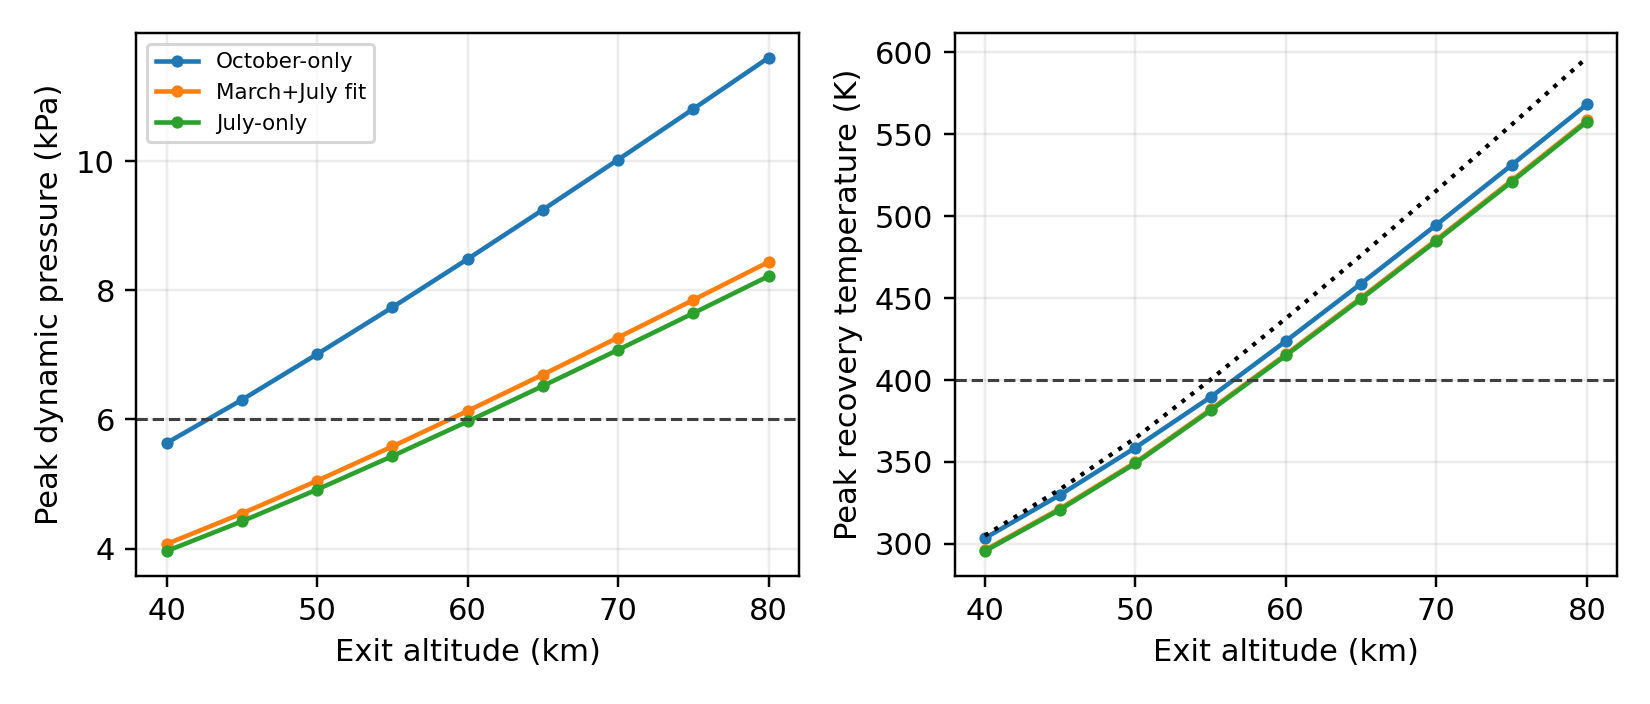
\includegraphics[width=.88\linewidth]{figures/loads_sweep.png}
\caption{Peak dynamic pressure and recovery-temperature proxy versus exit altitude for three transferred effective drag areas. Dashed lines mark assumed 6\,kPa and 400\,K screens; the dotted curve is the central case's stagnation-temperature proxy. None is a certified equipment limit.}
\end{figure}

\section{Risks, strengths, and next measurements}
The main dangers are thin-air attitude instability and flat spin; transonic and supersonic drag uncertainty; aerodynamic heating and localized fabric or visor hot spots; life-support or pressure loss; opening shock, line twist, or canopy failure; and a hard landing or unsuitable landing site. A vertical rocket release avoids orbital reentry speed, but an exit with appreciable horizontal rocket velocity would require a different trajectory and could dominate heating. At the highest modeled altitudes, the freefall part spends longer in very low density; the longer time affects oxygen and suit requirements even if the vertical dynamics remain tractable.

A minimal attitude model would require
\begin{equation}
I\dot\omega=qA\ell C_M(\alpha,M)-c_\omega\omega,
\qquad
a_{\rm head}\simeq \omega^2r_{\rm head},
\label{eq:spin}
\end{equation}
where $I$ is body-plus-equipment rotational inertia, $\ell$ an aerodynamic moment arm, $C_M$ a moment coefficient, $c_\omega$ rotational damping, and $r_{\rm head}$ the head's distance from the spin axis. These quantities and control-torque capacity are not identified by mass or vertical flight summaries. The Stratos report records an actual flat-spin episode, but its duration and forces cannot simply be scaled by an integral of downward drag acceleration \cite{stratos}. At a 60\,km exit the standard-atmosphere pressure is only about 22\,Pa, underscoring the need for a pressure suit and independent oxygen system throughout the fall.

The model's strengths are traceable public observations, an explicit speed calibration/holdout split, a separate drogue regime, units and numerical outputs that can be reproduced, and a maximum-altitude statement that exposes its assumptions. Its weaknesses are more consequential: the available published mission data are sparse summaries, the fixed drag area cannot represent body motion and compressibility, the standard atmosphere ignores actual weather, neither heat proxy is a material temperature, the canopy inflation law omits shock peaks, and no angular dynamics or medical tolerance model is fitted. The 42.7--57.8\,km spread is a sensitivity result under assumed thresholds, not a safety interval. Its proximity to any prior team's single numerical answer is not independent corroboration.

The most valuable validation data would be time-stamped altitude, velocity, attitude/spin rate, suit pressure and temperature, oxygen state, and parachute line-load traces from instrumented test drops. The published Stratos data support only pointwise vertical checks. A flight-ready conclusion would also need certified suit and parachute envelopes and a measured spin-control design.

\section{Conclusion}
With total mass 190\,kg alone, the requested maximum altitude is not identifiable. Under the stated standard-atmosphere model and illustrative 6\,kPa/400\,K equipment screens, the March--July drag-area fit gives approximately 57.7\,km. Substituting one-event effective drag areas from the other Stratos flights moves the same calculation to 42.7--57.8\,km; using a stagnation rather than turbulent recovery proxy moves the central 400\,K crossing from 57.7 to 55.0\,km. A 60\,km scenario has 639\,m\,s$^{-1}$ peak speed and 6.13\,kPa peak dynamic pressure, but neither these outputs nor a modeled landing speed establish survival. A defensible maximum requires a closed 190\,kg equipment design, rated heat and deployment limits, attitude-control and life-support data, and instrumented flight validation.

\begin{thebibliography}{99}\small
\bibitem{problem} University Physics Competition, \emph{2023 Contest: Problem A, Space Diving}. \url{https://www.uphysicsc.com/2023contest.html}.
\bibitem{rules} University Physics Competition, \emph{Contest Rules}. \url{https://uphysicsc.com/contestrules.html}.
\bibitem{tongji} Team 355, \emph{Maximum safe altitude for space jumps}, 2023. Supplied manuscript; public copy: \url{https://www.uphysicsc.com/2023-GM-A-355.pdf}.
\bibitem{team131} Team 131, \emph{2023 Problem A solution}. \url{https://www.uphysicsc.com/2023-GM-A-131.pdf}.
\bibitem{team227} Team 227, \emph{2023 Problem A solution}. \url{https://www.uphysicsc.com/2023-GM-A-227.pdf}.
\bibitem{team244} Team 244, \emph{2023 Problem A solution}. \url{https://www.uphysicsc.com/2023-GM-A-244.pdf}.
\bibitem{team447} Team 447, \emph{2023 Problem A solution}. \url{https://www.uphysicsc.com/2023-GM-A-447.pdf}.
\bibitem{team464} Team 464, \emph{2023 Problem A solution}. \url{https://www.uphysicsc.com/2023-GM-A-464.pdf}.
\bibitem{ussa} NOAA, NASA, and U.S. Air Force, \emph{U.S. Standard Atmosphere, 1976}. NASA Technical Reports Server, 1977. \url{https://ntrs.nasa.gov/citations/19770009539}.
\bibitem{stratos} Red Bull Stratos, \emph{Stratos Scientific Summit Report}, 2013, pp.~7, 10--11, 46. \url{https://lru.praxis.dk/Lru/microsites/hvadermatematik/hem3download/kap3a_QR20_ekstra_Report_Final.pdf}.
\bibitem{wyoming} University of Wyoming, Department of Atmospheric Science, \emph{Upper Air Sounding Archive}, stations 72364 and 72365, dated 2012 profiles. \url{https://weather.arcc.uwyo.edu/wsgi/sounding}.
\bibitem{guerster} M.~Guerster and U.~Walter, \emph{Aerodynamics of a highly irregular body at transonic speeds---Analysis of STRATOS flight data}, PLOS ONE, 2017. \url{https://journals.plos.org/plosone/article?id=10.1371/journal.pone.0187798}.
\bibitem{fai} FAI, \emph{Alan Eustace's High-Altitude Parachute Jump Records Still Stand}, 2024. \url{https://www.fai.org/news/yet-be-beaten-alan-eustaces-high-altitude-parachute-jump-records-still-stand-10-years}.
\bibitem{nasaopen} D.~W.~Way, \emph{A Momentum-Based Indicator for Predicting the Peak Opening Load of Supersonic Parachutes}, NASA Technical Reports Server, 2018. \url{https://ntrs.nasa.gov/citations/20180006292}.
\bibitem{nasahuman} NASA, \emph{Human Integration Design Handbook, Natural and Induced Environments}. \url{https://www.nasa.gov/reference/6-0-natural-and-induced-environments-vol-2/}.
\bibitem{spin} J.~M.~Pattarini et al., \emph{Flat spin and negative Gz in high-altitude free fall: pathophysiology, prevention, and treatment}, Aviation, Space, and Environmental Medicine, 2013. \url{https://pubmed.ncbi.nlm.nih.gov/24024308/}.
\end{thebibliography}
\end{document}
